% Created by Jiri Kubik, 2022
% '-> based on previous template by: Petr Cizek, 2018

% - frame -----------------------------------------------------------------
\begin{frame}
    \frametitle{Slide Layout -- Header and Footer}
    \begin{itemize}
        \item To configure slide layout, see {\tt main.tex}
        \item Use {\tt \textbackslash def\textbackslash compact\{1\}} place frame title to the slide header
        \item Use {\tt \textbackslash def\textbackslash compact\{0\}} place presentation name and author(s) to the slide header
        \item Use {\tt \textbackslash renewcommand\{\textbackslash footlineleft\}\{Footline Left Text\}}  to set ``Footline Left Text'' to the left footer part.
        \item Use {\tt \textbackslash renewcommand\{\textbackslash footlineright\}\{Footline Right Text\}}  to set ``Footline Left Text'' to the right footer part.
    \end{itemize}    
\end{frame}

% - frame -----------------------------------------------------------------
\begin{frame}
    \frametitle{Slide Content}
    \textctubf{Highlighting}
    \begin{itemize}
        \item Similarly to latex-based text commands, we provide them in ctu-blue:
        \begin{itemize}
            \item {\tt \textbackslash textbf\{\}} ... {\tt \textbackslash textctubf\{\}} for \textctubf{this effect},
            \item {\tt \textbackslash texttt\{\}} ... {\tt \textbackslash textctutt\{\}} for \textctutt{this effect},
            \item {\tt \textbackslash textit\{\}} ... {\tt \textbackslash textctuit\{\}} for \textctuit{this effect},
            \item {\tt \textbackslash emph\{\}} ... {\tt \textbackslash emphctu\{\}} for \emphctu{this effect},
            \item {\tt \textbackslash textnf\{\}} ... {\tt \textbackslash textctunf\{\}}, or just {\tt \textbackslash textctu\{\}} for \textctu{this effect}.
        \end{itemize}
    \end{itemize}
    \vspace{1em}
    \textctubf{Itemize and enumerate}
    \begin{columns}
        \begin{column}[]{0.3\textwidth}
            \begin{itemize}
                \item Level 1
                \begin{itemize}
                    \item Level 2
            	      \begin{itemize}
                        \item Level 3
                        \item Level 3
                    \end{itemize}
                    \item Level 2
        	    \end{itemize}
                \item Level 1   
           \end{itemize}
        \end{column}
        \begin{column}[]{0.3\textwidth}
            \begin{enumerate}
                \item Level 1
                \begin{enumerate}
                    \item Level 2
                    \begin{enumerate}
                        \item Level 3
                        \item Level 3
                    \end{enumerate}
                    \item Level 2
                \end{enumerate}
                \item Level 1
            \end{enumerate}
        \end{column}
        \begin{column}[]{0.3\textwidth}
            \begin{itemize}
                \item Level 1
                \begin{enumerate}
                    \item Level 2
                    \begin{itemize}
                        \item Level 3
                        \item Level 3
                    \end{itemize}
                    \item Level 2
                \end{enumerate}
                \item Level 1
            \end{itemize}
        \end{column}
    \end{columns}

\end{frame}

\begin{frame}
    \frametitle{References and Math}
    
    \textctubf{References}
    \begin{itemize}
        \item You can use a simple line reference, which saves space
        \item {\footnotesize \tt \textbackslash bibcit\{Author(s)\}\{Paper Title\}\{Conference/Journal\}\{Year[, Pages]\}}
    \end{itemize}
    \bibcit{Faigl J., Hollinger G.}{Unifying Multi-Goal Path Planning for Autonomous Data Collection}{IROS}{2014, 2937--2942.}
    
    \vspace{0.5em}
    \begin{itemize}
        \item Or one can use full bibliography entry (legacy) like
        \item {\footnotesize \tt \textbackslash bibligraphycitation\{Author(s)\}\{Paper Title\}\{Conference/Journal\}\{Year[, Pages]\}}
    \end{itemize}
    \bibligraphycitation{Faigl J., Hollinger G.}{Unifying Multi-Goal Path Planning for Autonomous Data Collection}{IROS}{2014, 2937--2942.}
    \vspace{1em}
    \textctubf{Math font testing}
    \begin{itemize}
        \item Use {\tt equation*} to disable numbering
        \begin{equation*}
            \dot{\mathbf{x}} = \mathbf{A}x + \mathbf{B}u,
        \end{equation*}
        \item where $x \in \mathbb{R}$
    \end{itemize}
    
    
\end{frame}


% - frame -----------------------------------------------------------------
\begin{frame}
    \frametitle{Embedded videos}
    \begin{itemize}
        \item For an embedded video to play you need:
        \begin{enumerate}
    	    \item video file in a directory \texttt{video}
    	    \item image file with the same resolution as video (screenshot) in a directory \texttt{fig}
    	    \item Okular pdf\footnote{https://okular.kde.org/cs/} viewer for the presentation
        \end{enumerate}
    \end{itemize}

    \begin{columns}
        \begin{column}[T]{0.5\textwidth}
            For example: \\
            \tt
            \textbackslash movie[width=0.8\textbackslash columnwidth, poster, autostart, loop]
            \{\\
                \textbackslash includegraphics[width=0.8\textbackslash columnwidth]
                \{fig/gait\}\\
            \}\\
            \{videos/gait\_sm.mp4\}
        \end{column}
        \begin{column}[T]{0.5\textwidth}
            \centering
            \movie[width=0.8\columnwidth, poster, autostart, loop]{
                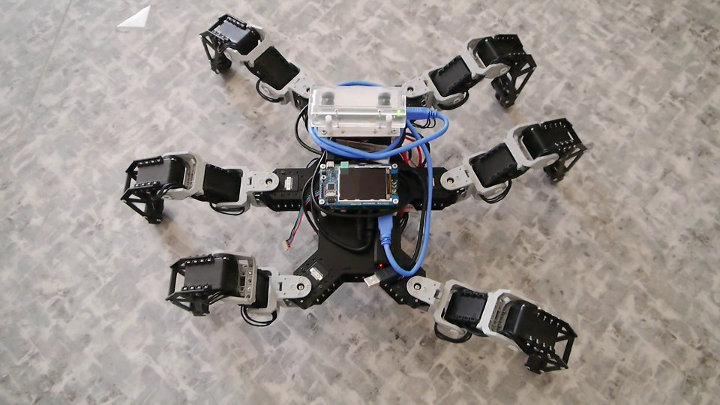
\includegraphics[width=0.8\columnwidth]{fig/gait}
            }
            {videos/gait_sm.mp4}
        \end{column}
    \end{columns}
\end{frame}

